Our approach for training RNNs is based entirely on the SGD framework described in Section~\ref{sec:sgd}. In particular we focus, separately, on the three main components of the algorithm, namely the initialization, the choice of the descent direction and the learning rate. We show that the initialization plays a crucial role in the learning process and can, alone, dictate if the learning process will be ``successful"\footnote{Here we refer to artificial tasks where a criterion for success is easily defined.} or not. We then propose a strategy to choose a descent direction to handle with the vanishing gradient. As for the learning rate, we use a technique which is entirely equivalent to the gradient clipping trick proposed in \cite{understandingExplodingGradients} which helps dealing with exploding gradients.


\section{Preliminaries}
Before focusing on each of the three above mentioned components we will introduce some notation needed in the following sections, as well as two artificial tasks which we will use as examples.
Recall from Section \ref{sec:rnn_intro} that each time step is associated with a loss function. It could be zero for all time steps but for the last, for example if we want to classify the whole sequences, or it could be defined for all the time steps if each intermediate output is relevant. Consider now a loss function $g$ for a generic time step $\tau$. Defining 
\begin{equation}
\nabla_{\mat{W^{rec}}} g_{|k}  \defeq \frac{\partial g}{\partial \vec{a}^{\tau}} \cdot \frac{\partial \vec{a}^{\tau}}{\partial \vec{a}^k} \cdot \frac{\partial^+ \vec{a}^k}{\partial \mat{W}^{rec}},
\end{equation}
and recalling the results of Section \ref{sec:rnn_grad}, we have
\begin{equation}
	\frac{\partial g_{\tau}}{\partial \mat{W}^{rec}} = \sum_{k=1}^{\tau} \nabla_{\mat{W^{rec}}} g_{|k}.
\end{equation}
Same definition applies for $\vec{b}_{rec}$ and $\mat{W}_{in}$. For $\mat{W}_{out}$ (and in an analogous way $\vec{b}_{out}$) we put
\begin{equation}
\nabla_{\mat{W^{out}}} g_{|k}  \defeq \frac{\partial g}{\partial \vec{z}^{\tau}} \cdot \frac{\partial^+ \vec{z}^k}{\partial \mat{W}^{out}}.
\end{equation}
We refer to $\nabla_{\vec{x}} g_{|k}$ as the temporal gradient for time step $k$ w.r.t. the variable $\vec{x}$, and it is easy to see that it is the gradient we would compute if we replicated the variable $\vec{x}$ for each time step and took the derivatives w.r.t. to its k-th replicate.

The \textbf{vanishing gradient} problem appears then, under this new notation, when the norm of the temporal components $\nabla_{\vec{x}} g_{|k}$ of recent time steps  are exponentially bigger than the ones of more distant ones.

The two tasks, designed to enhance the vanishing gradient problem, which we will use in the following are the \textit{addition} and the \textit{temporal order} tasks. They belong to a set tasks proposed by Hochreiter\cite{lstm} in 1991 and used as benchmarks ever since (see appendix \ref{app:tasks} for more details).

\paragraph{The Addition task.}
The input sequence is composed by an $\mathbb{R}^2$ vector. The first position is a marker which can be $0$ or $1$ and the second position is a real number in $(0,1)$. The goal is to predict the sum of the only two numbers marked with $1$. The task is difficult because such markers are placed one at the beginning and one at the end of very long sequences.

\begin{table}[h]
	\centering
\begin{tabular}{|c|c|c|c|c|c|c|c|c|c}
	\hline  marker & 0&  1&  0&  $\hdots$& 0 & 1 & 0 & 0  \\ 
	value & 0.3&  \textbf{0.7}&  0.1&  $\hdots$& 0.2& \textbf{0.4} & 0.6& 0.9  \\ 
	\hline 
\end{tabular}
\caption{An example for the addition task. The predicted output should be the sum (1.1) of the two one-marked positions.}
\label{table:add_example}
\end{table}


\paragraph{The Temporal order task}
The input sequence is composed of repetitions of six different symbols $\{a, b, c, d , x, y\}$.
There are only two $\{x, y\}$ symbols in the entire sequence. The goal of this task is to predict the relative order of such symbols, i.e. $\{xx, xy, yx, yy\}$, which as in the addition task, are one at the beginning and one at the end of the sequence.


\section{Initialization}
The first phase of the learning process is the initialization of the variables. We found that the choice of the initial value for the recurrent matrix $\mat{W_{rec}}$ has a big impact on the entire learning process. Recall the results from Section  \ref{sec:vanishing}, where we saw that having such a matrix with too small singular values, more precisely $\sigma'_{max} \cdot \mu_{max} <1 $, is a sufficient condition for the gradient to vanish. Although a sufficient condition that, instead, guarantees that the gradient does not vanish is not known, the bounds on the singular values encourage to explore initialization techniques which lead to matrices with higher singular values or higher spectral radius. A similar suggestion, motivated by other considerations, was given in the ESN field \cite{reservoirSummary}.

We propose an initialization scheme where the recurrent matrix is firstly sampled from a distribution\footnote{In all the experiments we always sampled from a zero mean Gaussian, but others distributions can be used as well.} and then scaled to have a specified spectral radius as shown in \ref{algo:init_scaling}.

\begin{algorithm}[!h]
	\KwData{\\
		\Indp
		$\rho = $ desired spectral radius
	}
	\BlankLine

	$\mat{W_{rec}} \sim \mathcal{N}(0, \sigma^2)$\\
	$r \gets \mbox{spectral\_radius}(\mat{W_{rec}})$\\
	$\mat{W_{rec}}\gets \frac{\rho}{r} \cdot \mat{W_{rec}}$\\
	\KwRet{$\mat{W_{rec}}$}
	\caption{Recurrent weight matrix initialization scheme}
	\label{algo:init_scaling}
\end{algorithm}

 In Figure \ref{fig:temporal_norms} we show, as an example, the temporal gradients, w.r.t. all the variables of the model, varying the spectral radius in [0.8, 0.9, 1, 1.1, 1.2], computed on a hundred samples for the temporal order task.

\begin{figure}
    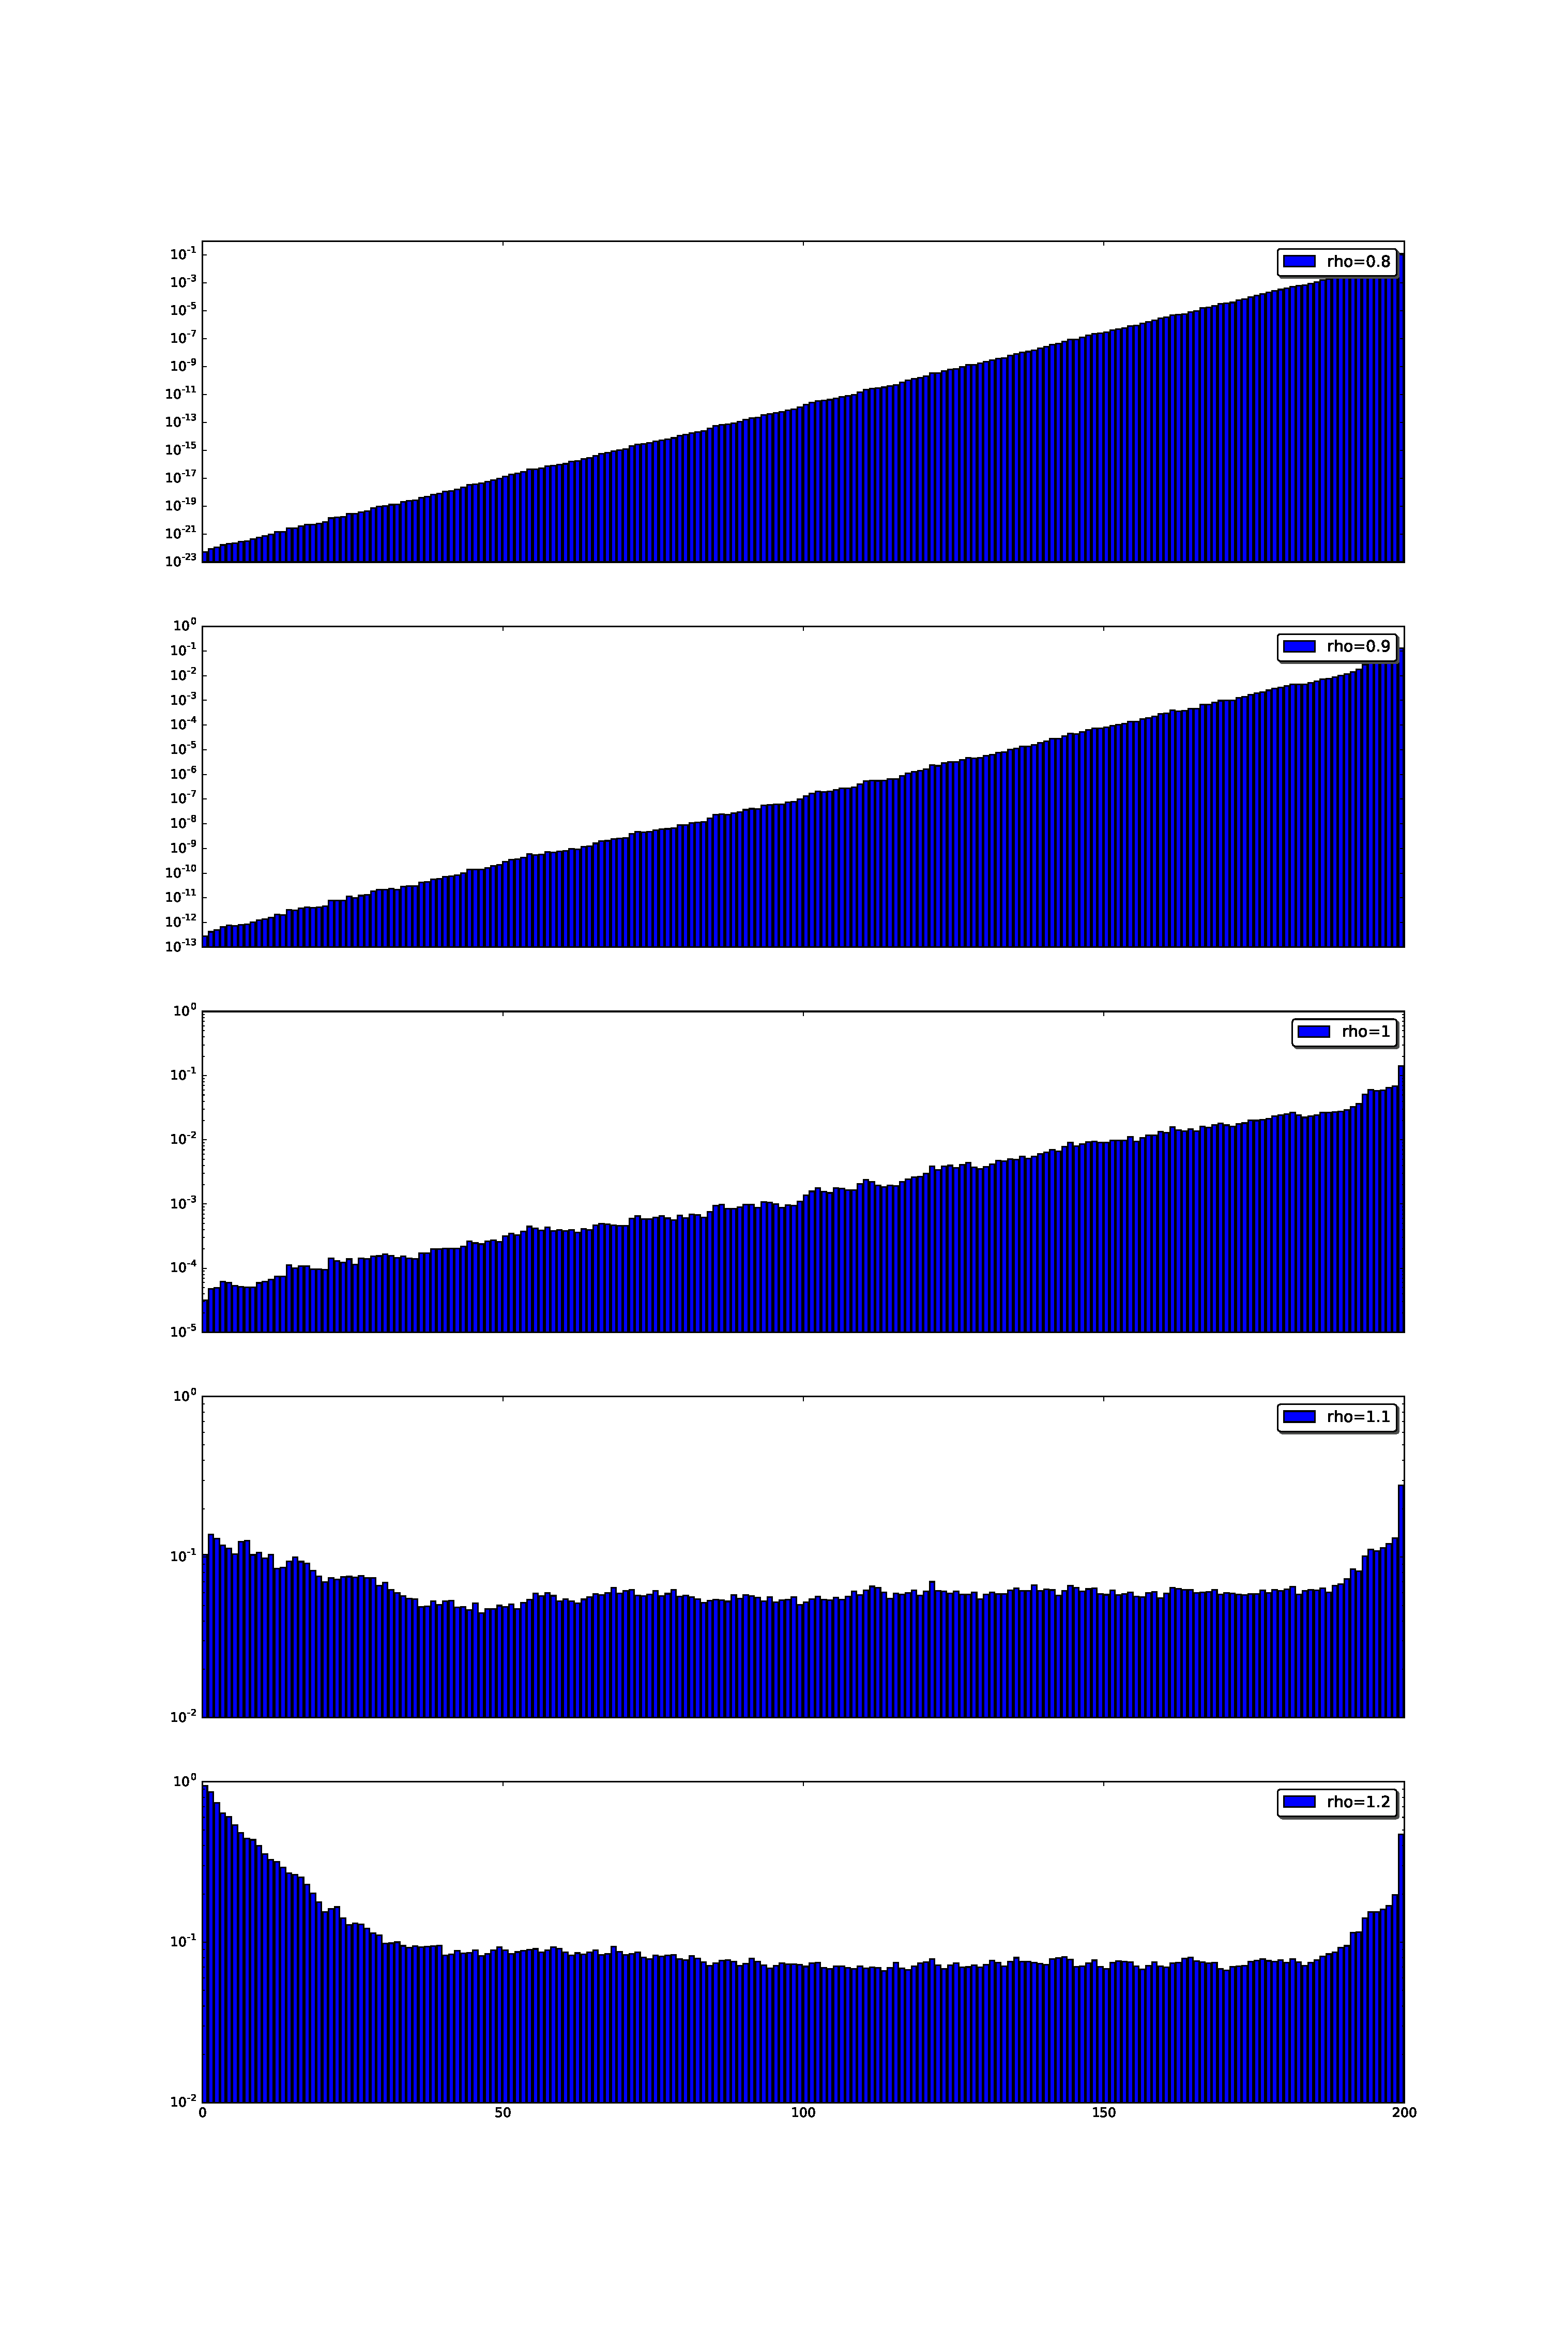
\includegraphics[width=0.9\textwidth]{chapter3/temporal_components.eps}
    \caption{Temporal gradients for the temporal order task varying the spectral radius of the recurrent matrix. y axis is in logarithmic scale.}
    \label{fig:temporal_norms}
\end{figure}

The first two cases, the one with spectral radius less than one, are perfect examples of vanishing gradient instances: more recent temporal components have norm exponentially larger than the more distant ones (please note that the y axis is in logarithmic scale). On the contrary such phenomenon is not observed in the cases of spectral radius larger than one where the temporal components have roughly the same norm.

We found that, at least in the task we explored, an appropriate spectral radius always allows the training process to start in a regime where the gradient does not vanish. We report some results on the effect of the initialization on the training process in Chapter \ref{ch:experiments}.

\section{Descent direction}
In the previous section we have seen how providing a proper initialization of the recurrent matrix can lead to a starting point where gradient does not vanish. However, no matter how we choose the starting point, we have no guarantees that the gradient will not vanish after some iterations. In Figures \ref{fig:comparison_add_temp_0} and \ref{fig:comparison_add_temp_1}, we compare the temporal gradients of two different tasks (the addition and the temporal order ones) at the beginning and after a few iterations.
We notice that, although they have comparable temporal gradients norms at the beginning, they behave very differently after a few iterations: in the case of the addition task we can surely say that after a few iterations the gradient start to vanish.

\begin{figure}[h]
	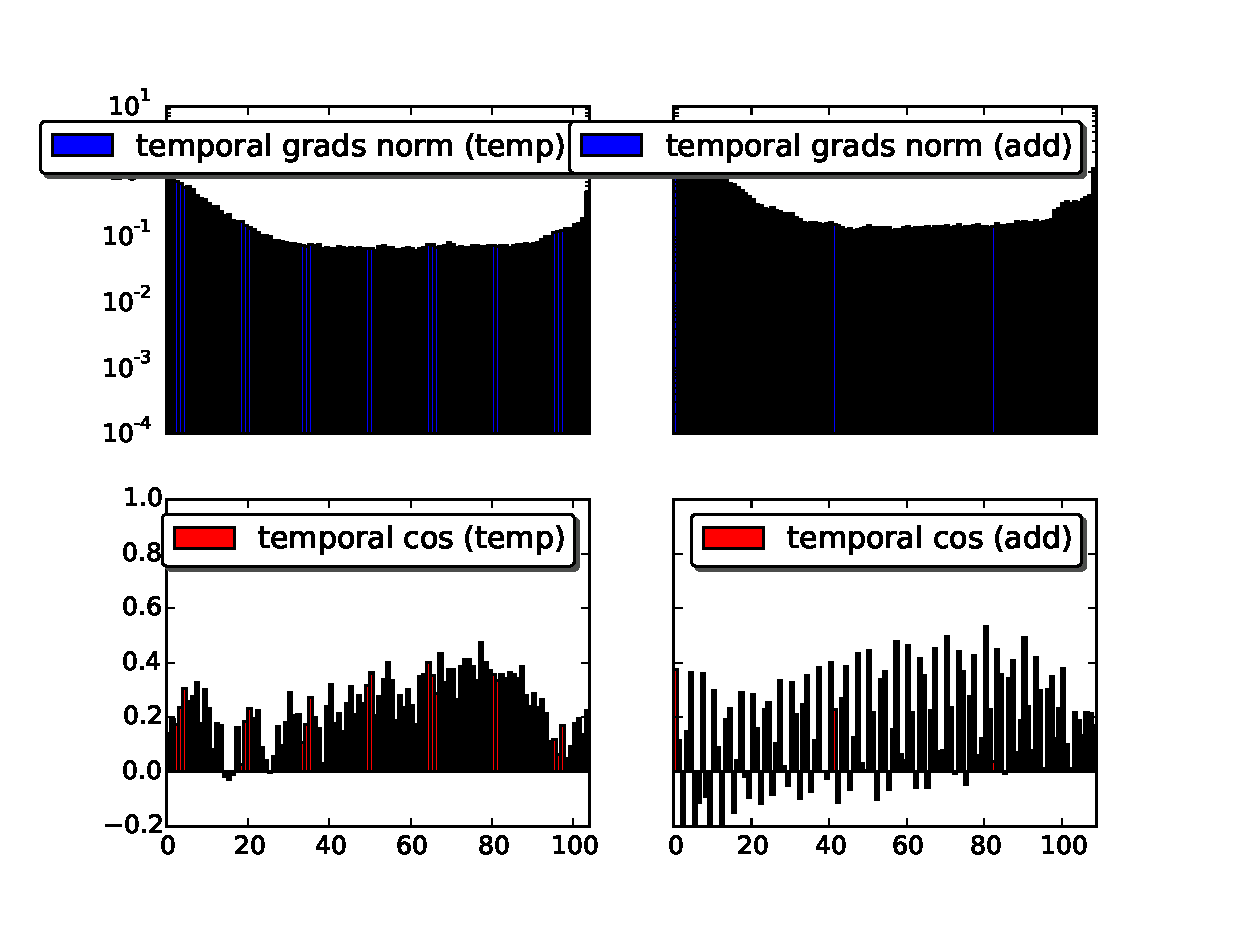
\includegraphics[width=1\textwidth]{chapter3/compare_add_temp_norms_0.eps}
	\caption{Comparison between the temporal order task (first column) and the addition task (second column). First row shows the norms of the temporal gradients, while the second shows the cosine between each temporal component and the gradient. This is a snapshot taken at the first iteration of the training process.}
	\label{fig:comparison_add_temp_0}
\end{figure}

\begin{figure}[h]
	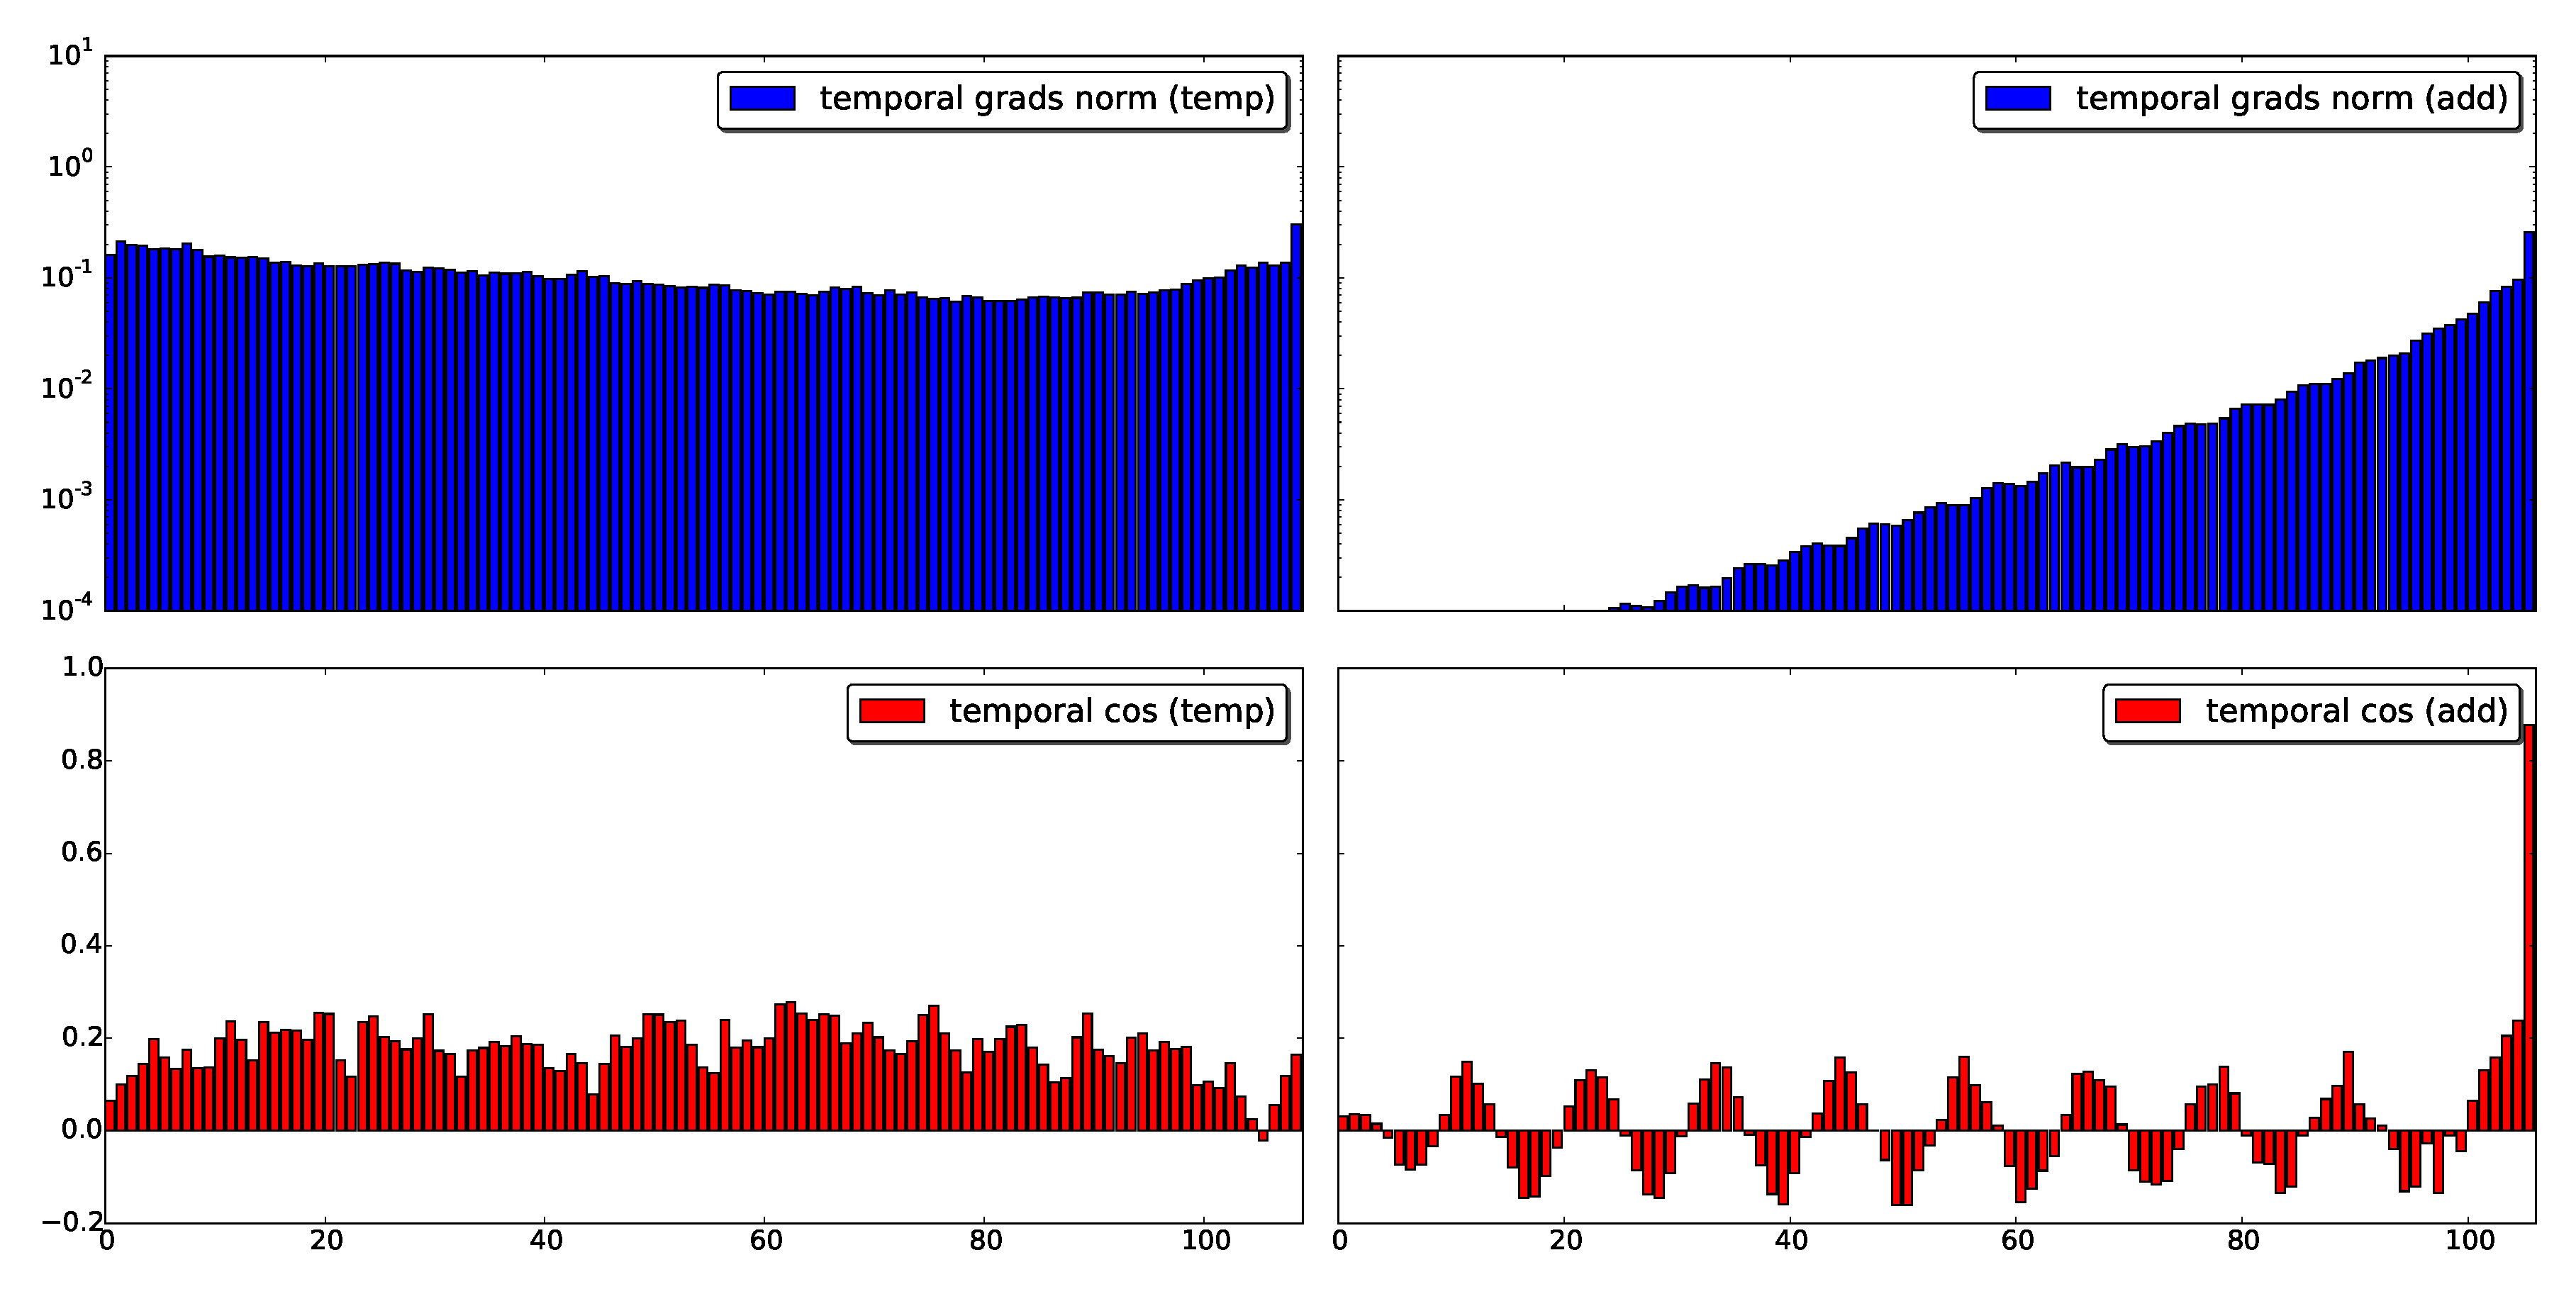
\includegraphics[width=1\textwidth]{chapter3/compare_add_temp_norms_1.eps}
	\caption{Caption as in Figure \ref{fig:comparison_add_temp_0}. This is a snapshot taken after a few iterations of the training process.}
	\label{fig:comparison_add_temp_1}
\end{figure}


Motivated by this, we introduce a new descent direction, which we will call the \textit{simplex direction},
which should not suffer from the vanishing problem. In the following we will consider only the case where there is a single loss function $L$ on the last time step, as in the artificial tasks, but the approach is easily generalizable to problems where a loss function is defined also for the intermediate time steps. The simplex direction is obtained by the following steps:


\begin{itemize}
	\item Normalize the temporal gradients:
	\begin{equation}
	s_t(\vec{x}) = \frac{\nabla L_{|t}(\vec{x})}{\norm{\nabla L_{|t}(\vec{x})}}.
	\end{equation}
	
	\item Combine the normalized gradients in a convex way:
	\begin{equation}
	s(\vec{x}) = \sum_{t=1}^T \beta_t \cdot s_t(\vec{x}).
	\end{equation}
	
	with $\sum_{t=1}^T\beta_t=1, \beta_t>0$ (randomly picked at each iteration).
	\item Introduce the gradient norm:
	\begin{equation}
	d(\vec{x}) = - \norm{\nabla L (\vec{x})}\frac{s(\vec{x})}{\norm{s(\vec{x})}}.
	\end{equation}
\end{itemize}

As we have seen in Section \ref{sec:rnn_grad} the anti-gradient direction is the sum of all temporal gradients. The idea is to combine the gradients in such a way that the gradient contains information about all time steps, i.e. does not suffer from the vanishing problem. This is achieved by normalizing all the temporal gradients. The idea to combine them in a convex, simplex-type way, as suggested by some numerical evidence, adds some robustness to the method. Finally since we discard any information about the norms in the normalization process, we choose to give the simplex direction the norm of the gradient. In this way we can see the obtained direction as a projection of the gradient.


\section{Learning rate}

The choice of the learning rate is crucial for the success of the training procedure. It is well known that RNNs give rise to gradients which change extremely fast in norm (the exploding gradient problem). This makes choosing a single constant step, or even designing an adaptive strategy, very difficult, at the least, for this kind of models. A simple trick which allow to choose a fixed step from the beginning is to \textit{clip the gradients}. This technique was introduced and used in slightly different forms in \cite{understandingExplodingGradients} and \cite{clippingMikolov} and we described it in Section \ref{sec:clipping}. We reformulate the version proposed in \cite{understandingExplodingGradients} as a learning rate selection strategy.
Given a direction $\vec{d}_k$ the step $\alpha_k$ is chosen as:
\begin{equation}
\alpha_k = 
\begin{cases}
	\mu  \quad &\mbox{if} \norm{\vec{d}_k}_2 \leq \tau\\
	\frac{\mu \cdot \tau}{\norm{\vec{d}_k}_2} \quad & otherwise,
\end{cases}
\end{equation}
where $\mu$ and $c$ are some positive constants. The parameter $\tau$ is the threshold on the direction norm; $\mu$, instead, is the constant learning rate that is used when the norm of the direction is not above such threshold. The idea is to use a constant step when the direction has small enough norm and vice-versa choose a step which is inversely proportional when such norm is too large. We confirm, as found in works cited above, that this trick is essential to train RNNs in a stochastic framework.

\section{Putting all together}
Now that we have described all the three main components of the algorithm we can put them together, as we do in Algorithm \ref{algo:complete_solution}, but with an important additional feature. The idea is to use the simplex combination at the beginning of the training process, or whenever the gradient is vanishing, and switch back to the anti-gradient when appropriate. This is done by checking the norm of the gradient, as in Line \ref{algo:line:condition}.


\begin{algorithm}[]
	\KwData{\\
		\Indp
		$D=\{\pair{\vec{x}^{(i)}}{\vec{y}^{(i)}}\}$: training set\\
		$m$: size of each mini-batch\\
		$\mu$: constant learning rate\\
		$\tau$: gradient clipping threshold \\
		$\rho$: initial spectral radius \\
		$\psi$ threshold for the direction norm
	}
	
	\KwResult{\\
		\Indp $\theta$: solution
	}
	\BlankLine
	
	$\mat{W_{rec}}, \mat{W_{in}, \mat{W_{out}}} \sim \mathcal{N}(0, \sigma^2)$\\
	$\vec{b}_{out}, \vec{b}_{rec} \gets 0$\\
	$r \gets \mbox{spectral\_radius}(\mat{W_{rec}})$\\
	$\mat{W_{rec}}\gets \frac{\rho}{r} \cdot \mat{W_{rec}}$\\
	$\theta_0 = [\mat{W_{rec}}, \mat{W_{in}}, \mat{W_{out}},\vec{b}_{out}, \vec{b}_{rec}]$

	
	\BlankLine
	\While{stop criterion}{
		
		$I$ $\gets$ sample $m$ training example $\in D$  \\
		$\{\nabla_\theta L_{|t}\}_{t=1}^{T} \gets \mbox{compute\_temporal\_gradients}(\theta_k, I)$\\
		\tcc{T is the length of the sequences. All sequences in a batch have the same length}
		$\vec{d}_k \gets \mbox{simplex\_combination}(\{\nabla_\theta L_{|t}\})$\\
		
		\If{$\norm{\nabla_{\theta}L(\theta_k)}_2 > \psi$}
			{$\vec{d}_k \gets \nabla_{\theta}L(\theta_k)$ \\
			\label{algo:line:condition}
		}
		
		$\alpha_k = 
		\begin{cases}
			\mu  \quad &\mbox{if} \norm{\vec{d}_k}_2 \leq \tau\\
			\frac{\mu \cdot \tau}{\norm{\vec{d}_k}_2} \quad & \mbox{otherwise}
		\end{cases}$\\
		
		$\theta_{k+1} \gets \theta_k + \alpha_k \vec{d}_k$\\
		$k\gets k+1$
	}
	\KwRet{$\theta_k$}
	\caption{RNN training}
	\label{algo:complete_solution}
\end{algorithm}

\section{Proof of convergence}
 
\documentclass{article}
\usepackage[utf8]{inputenc}
\usepackage[italian]{babel}
\usepackage{graphicx}
\usepackage{cite}
\usepackage[hidelinks]{hyperref}
\usepackage{listings}
\usepackage{latexsym}
\usepackage{amsmath}
\usepackage{proof}
\usepackage{stmaryrd}
\usepackage{amssymb}
\usepackage{epstopdf}
\usepackage{pgf}
\usepackage{tikz}
\usepackage[noend]{algpseudocode}
\usepackage[ruled,noline,linesnumbered]{algorithm2e}
\usetikzlibrary{automata,arrows}
\let\emptyset\varnothing

\graphicspath{ {./images/} }

%%Notation:

%%vectors
\renewcommand{\vec}[1]{\boldsymbol{#1}}
%%sets
\newcommand{\set}[1]{\mathcal{#1}}
%%matrixes
\newcommand{\mat}[1]{#1}
%%norm
\newcommand{\norm}[1]{\left\Vert #1 \right\Vert}
%%defeq
\newcommand{\defeq}{\triangleq}
%%
\newcommand{\net}[1]{\mathrm{#1}}
%% pair<x,y>
\newcommand{\pair}[2]{\langle#1,#2\rangle}

\title{Stochastic gradient descent}
\author{Giulio Galvan}

\begin{document}
	\maketitle
\noindent
Consider the stochastic optimization problem 
\begin{equation}
	\underset{\vec{x} \in \mathbb{R}^n}{\text{min}} f(\vec{x}) = \mathbb{E[F(\vec{x}, \vec{\xi})]},
	\label{eq:stochastic_prob}
\end{equation}
where $\vec{\xi} \in \Omega \subset \mathbb{R}^d$ is a random vector.
Suppose $f(\cdot)$ is continuous, strongly convex (with constant $c$) and there exists a compact level set of $f(\cdot)$, hence (\ref{eq:stochastic_prob}) has a unique optimal solution $\vec{x}_*$. Let also $L$ be the Lipschitz constant of $\nabla f$.
We make the following two assumptions:
\begin{itemize}
	\item	It is possible to generate independent identically distributed samples of $\vec{\xi}$
	\item There exists an oracle which, for a given point $(\vec{x}, \vec{\xi})$ return a stochastic descent direction $D(\vec{x}, \vec{\xi})$ such that $d(\vec{x})\defeq\mathbb{E}[D(\vec{x}, \vec{\xi})]$ satisfies:
	\begin{equation}
	-(\vec{x}-\vec{x}_*)^T (\nabla f(\vec{x}) -g(\vec{x})) \geq -\mu L \norm{\vec{x}_j-\vec{x}_*}^2_2\quad \forall \vec{x} \in \mathbb{R}^n,
	\label{eq:angular_condition}
	\end{equation}
	for some $\mu \in (0,\frac{c}{L}) $.
\end{itemize}
Consider the algorithm defined by
\begin{equation}
	\vec{x}_{j+1} = \vec{x}_j -\gamma_j D(\vec{x}_j,\vec{\xi}_j).
	\label{eq:stochastic_algo}
\end{equation}
Each iterate $\vec{x}_j$ of such random process is a function of the history $\vec{\xi}_{[j-1]}=(\vec{\xi}_1,\dots, \vec{\xi}_{j-1})$

Let $A_j\defeq \norm{\vec{x}_j-\vec{x}_*}^2_2$ and $a_j\defeq\mathbb{E}[A_j]$.
From (\ref*{eq:stochastic_algo}) we get
\begin{equation}
\begin{aligned}
	A_{j+1} &= \frac{1}{2}\norm{\vec{x}_j - \gamma_jD(\vec{x}_j,\vec{\xi}_j) -\vec{x}_*}^2_2\\ 
	&= A_j +\frac{1}{2}\gamma_j^2\norm{D(\vec{x}_j,\vec{\xi}_j)}^2_2 - \gamma_j(\vec{x}_j-\vec{x}_*)^TD(\vec{x}_j,\vec{\xi}_j).
\end{aligned}
\label{eq:aj_rec}
\end{equation}
Since $\vec{x}_j = \vec{x}_j(\vec{\xi_{[j-1]}})$ is independent of $\vec{\xi}_j$ we have
\begin{equation}
\begin{aligned}
	\mathbb{E}_{\vec{\xi}_{[j]}}[(\vec{x}_j-\vec{x}_*)^TD(\vec{x}_j,\vec{\xi}_j)] &= \mathbb{E}_{\vec{\xi}_{[j-1]}}[\mathbb{E}_{\vec{\xi}_{[j]}}[(\vec{x}_j-\vec{x}_*)^TD(\vec{x}_j,\vec{\xi}_j)]|\vec{\xi}_{[j-1]}]\\
	&= \mathbb{E}_{\vec{\xi}_{[j-1]}}[(\vec{x}_j-\vec{x}_*)^T\mathbb{E}{\vec{\xi}_{[j]}}[D(\vec{x}_j,\vec{\xi}_j)]|\vec{\xi}_{[j-1]}]\\
	&=\mathbb{E}_{\vec{\xi}_{[j-1]}}[(\vec{x}_j-\vec{x}_*)^Td(\vec{x}_j)]\\
\end{aligned}
\label{eq:independece}
\end{equation}
Let now assume that there exists $M>0$ such that
\begin{equation}
	\mathbb{E}[\norm{D(\vec{x},\vec{\xi})}^2_2]\leq M^2 \quad \forall \vec{x} \in \mathbb{R}^n.
	\label{eq:gradient_bound}
\end{equation}
Using (\ref{eq:independece}) and (\ref{eq:gradient_bound}) we obtain, taking expectation of both sides of (\ref{eq:aj_rec})
\begin{equation}
	a_{j+1} \leq a_j - \gamma_j\mathbb{E}_{\vec{\xi}_{[j-1]}}[(\vec{x}_j-\vec{x}_*)^Td(\vec{x}_j)] + \frac{1}{2}\gamma_j^2M^2
	\label{eq:aj_rec_2}
\end{equation}
Since $f(\cdot)$ is strongly convex there exists $c>0$ such that
\begin{equation}
	(\vec{y}-\vec{x})^T(\nabla f(\vec{y})- \nabla f(\vec{x}))\geq c \norm{\vec{y}-\vec{x}}^2_2
	\label{eq:strong_convexity}
\end{equation}
By optimality of $\vec{x}_*$ we have
\begin{equation}
	(\vec{x}-\vec{x}_*)^T\nabla f(\vec{x}_*) \geq 0 \quad \vec{x} \in \mathbb{R}^n.
	\label{eq:optimality}
\end{equation}
Inequalities (\ref{eq:optimality}) and (\ref{eq:strong_convexity}) implies
\begin{equation}
	(\vec{x}-\vec{x}_*)^T \nabla f(\vec{x}) \geq c \norm{\vec{x}-\vec{x}_*}^2_2 \quad \vec{x} \in \mathbb{R}^n.
\end{equation}
Adding and subtracting the descent direction $g(\vec{x})$ we get
\begin{equation}
	(\vec{x}-\vec{x}_*)^T (\nabla f(\vec{x}) -g(\vec{x}) +g(\vec{x})) \geq c \norm{\vec{x}-\vec{x}_*}^2_2,
\end{equation}
which can be rewritten as
\begin{equation}
		(\vec{x}-\vec{x}_*)^T g(\vec{x}) \geq c \norm{\vec{x}-\vec{x}_*}^2_2 - (\vec{x}-\vec{x}_*)^T (\nabla f(\vec{x}) -g(\vec{x}))
		\label{eq:angular_inequality}
\end{equation}
From assumption (\ref{eq:angular_condition}), taking expectations of both side of (\ref{eq:angular_inequality}) we obtain
\begin{align}
\mathbb{E}[(\vec{x}_j-\vec{x}_*)^T g(\vec{x}_j)] &\geq c \mathbb{E}[\norm{\vec{x}_j-\vec{x}_*}^2_2)] - \mathbb{E}[(\vec{x}_j-\vec{x}_*)^T (\nabla f(\vec{x}_j) -g(\vec{x}_j))]\\
 &\geq c(1-\frac{\mu L}{c}) \mathbb{E}[\norm{\vec{x}_j-\vec{x}_*}^2_2)]\\
 & = 2\bar{c}a_j,
\end{align}
with $\bar{c}=c(1-\frac{\mu L}{c})$.
Hence from (\ref{eq:aj_rec_2}) follows 
\begin{equation}
	a_{j+1} \leq (1-2\bar{c}\gamma_j)a_j + \frac{1}{2}\gamma_j^2M^2.
\end{equation}
Choosing the stepsizes as $\gamma_j = \frac{\beta}{j}$ for some constant $\beta>\frac{1}{2\bar{c}}$ we get
\begin{equation}
		a_{j+1} \leq (1-2\bar{c}\gamma_j)a_j + \frac{1}{2}\frac{\beta^2M^2}{j^2}.
\end{equation}
It follows by induction that
\begin{equation}
	\mathbb{E}[\norm{\vec{x}_j - \vec{x}_*}^2_2] = 2a_j\leq \frac{Q(\beta)}{j},
\end{equation}
where 
\begin{equation}
	Q(\beta) = max\left\{\frac{\beta^2M^2}{2\bar{c}-1},\norm{\vec{x}_1 - \vec{x}_*}^2_2 \right\}.
\end{equation}
Hence, since
\begin{equation}
	f(\vec{x})\leq f(\vec{x}_*) + \frac{1}{2}L\norm{\vec{x} - \vec{x}_*}^2_2, \quad \forall \vec{x} \in \mathbb{R}^n,
\end{equation}
we obtain
\begin{equation}
	\mathbb{E}[f(\vec{x}_j)-f(\vec{x}_*)] \leq \frac{1}{2} L \mathbb{E}[\norm{\vec{x}_j - \vec{x}_*}^2_2] \leq \frac{1}{2}LQ(\beta)
\end{equation}

\paragraph{Sufficient descent direction condition} Assumption \ref{eq:angular_condition} can be further elaborated.
Let $\theta$ be the angle between $\nabla f(\vec{x})$ and $g(\vec{x})$ and $\norm{g(\vec{x})} = \alpha \norm{\nabla f(\vec{x})}$ for some $\alpha>0$.
Then,
\begin{align}
	\norm{\nabla f(\vec{x}_j)-g(\vec{x}_j)}^2 &= \norm{\nabla f(\vec{x}_j)}^2 + \norm{g(\vec{x}_j)}^2 -2\norm{\nabla f(\vec{x}_j)}\norm{g(\vec{x}_j)}\cos\theta_j\\
	&=  \norm{\nabla f(\vec{x}_j)}^2(1+\alpha_j^2-2\alpha_j \cos\theta_j).
\end{align}
Since $\nabla f(\vec{x}_*)=0$, using Lipschitz continuity of $\nabla f$ (with constant L) we get
\begin{equation}
	\norm{\nabla f(\vec{x}_j)-g(\vec{x})} \leq L\norm{\vec{x}-\vec{x}_*} (1+\alpha^2-2\alpha \cos\theta)^{\frac{1}{2}}
\end{equation}
Hence
\begin{align}
(\vec{x}-\vec{x}_*)^T (\nabla f(\vec{x}) -g(\vec{x})) &\leq \norm{\vec{x}-\vec{x}_*} \norm{\nabla f(\vec{x}) -g(\vec{x})}\\
&\leq L\norm{\vec{x}-\vec{x}_*}^2 (1+\alpha^2-2\alpha \cos\theta)^{\frac{1}{2}}.
\end{align}
Hence a sufficient condition for assumption \ref{eq:angular_condition} to hold is
\begin{equation}
	1+\alpha^2-2\alpha \cos\theta_j\leq \mu^2
\end{equation}

\end{document}      



